\setAuthor{Andreas Valdmann}
\setRound{lõppvoor}
\setYear{2014}
\setNumber{G 4}
\setDifficulty{5}
\setTopic{Geomeetriline optika}

\prob{Periskoopprillid}
\begin{wrapfigure}{r}{0.38\textwidth}
 \begin{center}
 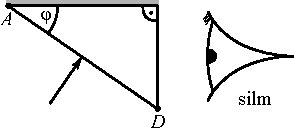
\includegraphics[width=0.4\textwidth]{2014-v3g-04-periskoopprillid_yl_joonis.pdf}
 \end{center}
\end{wrapfigure}

Kui liiga kaua järjest raamatut lugeda, võib kael pikast allapoole vaatamisest ära väsida. Selle vältimiseks on välja mõeldud erilised prillid, mille abil saab pead kallutamata alla vaadata. Prillide põhiliseks elemendiks on joonisel kujutatud prisma, mille pealmine tahk on kaetud valgust peegeldava materjaliga. Prisma tipunurk $\varphi$ on valitud selliselt, et kui prismasse sisenev valguskiir on pinnaga risti, siis on seda ka väljuv kiir. Prisma on tehtud materjalist murdumisnäitajaga $n=\SI{1,5}{}$. 

\osa Lõigul $AD$ on punktid $B$ ja $C$, mis jagavad selle kolmeks piirkonnaks: $AB$, $BC$ ning $CD$. Sõltuvalt sellest, millisele piirkonnale kiir langeb, on kiire käiguks prismas kolm põhimõtteliselt erinevat võimalust. Tehke joonis kiirte käigust kõigi juhtude jaoks.\\
\osa Leidke nurga $\varphi$ väärtus.\\
\osa Olgu külje $AD$ pikkus $l$. Kui kaugel asuvad punktid $B$ ja $C$ tipust $A$?\\
\osa Miks on prillides üldsegi vaja kasutada suhteliselt keerulist prismaga süsteemi, selle asemel et kiirte kallutamiseks kasutada ühte tasapeeglit?

\hint
Nurga $\varphi$ leidmiseks tuleb vaadelda kiirt, mis siseneb lõiku $AB$.

\solu
\osa Kuna sisenevad ja väljuvad kiired on prisma pinnaga risti, siis keskkondade lahutuspiiril nende suund ei muutu. Kui kiir langeb prismale lõigul $AB$, siis peegeldub see esmalt prisma ülemisel tahul, seejärel alumisel tahul ning väljub prismast läbi parempoolse tahu (vt joonist). Kui kiir langeb prismale lõigul $BC$, siis peegeldub see ülemisel tahul, siis parempoolsel tahul ning väljub läbi alumise tahu ja ei jõuagi silma. Kui kiir langeb prismale lõigul $CD$, siis peegeldub see esmalt parempoolsel tahul, seejärel ülemisel tahul ning väljub jällegi läbi alumise tahu.

\begin{center}
 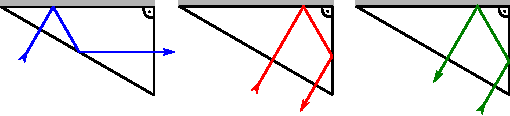
\includegraphics[width=0.8\textwidth]{2014-v3g-04-periskoopprillid_lahendus_joonis1.pdf}
\end{center}

\osa Vaatleme kiirt, mis siseneb prismasse lõigul $AB$. Kuna sisenev kiir on pinnaga risti, siis tekib täisnurkne kolmnurk $AKL$ (vt joonist). Kolmnurga üheks teravnurgaks on $\varphi$ ja seega on teise teravnurga suurus $\ang{90}-\varphi$. Kuna viimane nurk on esimesel peegeldumisel langemisnurga täiendnurgaks, siis on ka langemisnurk $\varphi$. Peegeldumisseadusest järeldub, et esimene peegeldumisnurk on samuti $\varphi$. Kuna prismast väljuv kiir on paralleelne prisma ülemise tahuga, siis on teisel peegeldumisel peegeldumisdumisnurga täiendnurk ja seega ka langemisnurga täiendnurk $\varphi$. Näeme, et täisnurkse kolmurga $KLM$ teravnurgad on $\varphi$ ja $2\varphi$. Kuna kolmnurga sisenurkade summa on \ang{180}, siis $\varphi=(\ang{180}-\ang{90})/3=\ang{30}$.

\begin{center}
 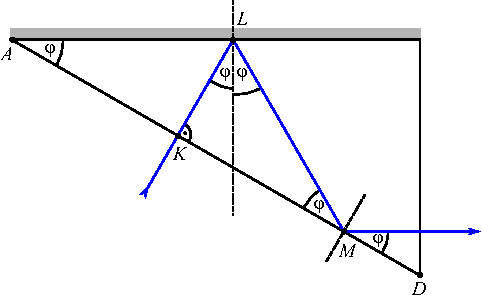
\includegraphics[width=0.65\textwidth]{2014-v3g-04-periskoopprillid_lahendus_joonis2.pdf}
\end{center}

\emph{Märkus.} Nüüd, kui prisma tipunurk on leitud, saame veenduda, et kui pinnaga risti sisenenud kiir peegeldub prisma alumiselt või parempoolselt tahult, siis on need peegeldumised täielikud. Eelmisest alaülesandest on näha, et nendel juhtudel on langemisnurgaks $\ang{90}-\varphi=\ang{60}$. Täieliku sisepeegeldumise piirnurk on $\alpha=\arcsin(1/n)=\ang{42}$. Langemisnurk \ang{60} on sellest suurem ehk toimub täielik sisepeegeldumine.

\osa Kui kiir siseneb prismasse punktis $B$, siis läbib väljuv kiir punkti $D$ (vt joonist).

\emph{Märkus.} Väljuva kiire suund pole sel juhul üheselt määratud, kuid see ei oma ülesande lahendamisel tähtsust.\\
Kasutades eelmises alaülesandes saadud $\varphi$ väärtust, on näha, et kolmnurgad $ABL$ ja $BDL$ on teineteise peegeldused lõigu $BL$ suhtes (öeldakse, et need kolmnurgad on kongruentsed). Seega on lõikude $AB$ ja $BD$ pikkused võrdsed, millest järeldub, et $|AB|=l/2$. Kui kiir siseneb prismasse punktis $C$, siis peegeldub see punktis $O$ otse tagasi ning väljub prismast punktis $C$. Täisnurksetest kolmnurkadest saame, et $|AO|=\cos(\ang{30})|AD|$ ja $|AC|=\cos(\ang{30})|AO|$ ehk punkti $C$ kaugus punktist $A$ on 
\[
|AC|=\cos^2(\ang{30})|AD|=\frac{3}{4}l.
\]

\begin{center}
 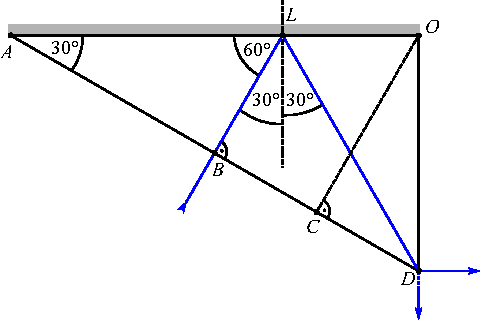
\includegraphics[width=0.65\textwidth]{2014-v3g-04-periskoopprillid_lahendus_joonis3.pdf}
\end{center}

\osa Ühe tasapeegli kasutamisel paistab tekst peegelpildis. Seetõttu tuleb teksti õigetpidi nägemiseks kasutada süsteemi, kus toimub paarisarv peegeldusi.

\probeng{Periscope glasses}
\begin{wrapfigure}{r}{0.38\textwidth}
  \begin{center}
    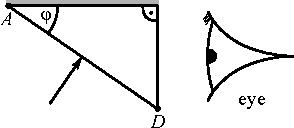
\includegraphics[width=0.4\textwidth]{2014-v3g-04-periskoopprillid_yl_joonis_ing}
  \end{center}
\end{wrapfigure}
Reading a book for too long is known to cause neck strain. To avoid this, a special pair of glasses were invented that do not require tilting the head to look down. The main element of these glasses is a prism shown in the figure. The upper face of the prism is covered with a material that reflects light. The apex angle $\varphi$ of the prism is chosen so that if the light ray entering the prism is perpendicular to the surface, then the ray that exits is also perpendicular. The prism is made of material with a refractive index $n=\SI{1,5}{}$.\\
a) On the line $AD$ there are points $B$ and $C$ that divide it into three sections: $AB$, $BC$ and $CD$. Depending on what section the ray falls on there are in principal three different routes in the prism for the ray. Make a draft of the ray’s routes for all the cases. \\
b) Find the value of $\varphi$.\\
c) Let the length of the side $AD$ be $l$. How far are the points $B$ and $C$ distanced from the tip $A$?\\
d) Why is this quite complex system used in the glasses instead of using a simple plane mirror to tilt the beams?

\hinteng
To find the angle $\varphi$ you should observe the ray that enters the section $AB$.

\solueng
\osa Because the entering and exiting rays are perpendicular to the surface of the prism then their direction does not change on the separation surface of environments. If a ray falls on the prism on the section $AB$ then it first reflects on the upper face of the prism, next on the bottom face and exits from the prism through the right face (see figure). If a ray falls on the prism on the section $BC$ then it reflects on the upper face, then on the right face, after that exits through the bottom face and does not reach the eye. If a ray falls on the prism on the section $CD$ then it first reflects on the right face, then on the upper face and exits again through the bottom face. 
\begin{center}
  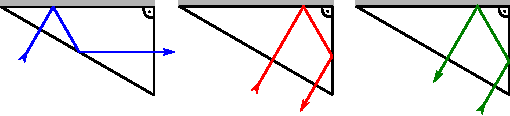
\includegraphics[width=0.8\textwidth]{2014-v3g-04-periskoopprillid_lahendus_joonis1}
\end{center}
\osa Let us observe a ray that enters the prism on the section $AB$. Because the entering ray is perpendicular to the surface a right triangle $AKL$ is formed (see figure). One of the acute angles of the triangle is $\varphi$ and therefore the value of the other acute angle is $\ang{90}-\varphi$. Because the latter angle is the supplementary angle for the angle of incidence of the first reflection then the angle of incidence is also $\varphi$. From the law of reflection it is concluded that the first angle of reflection is also $\varphi$. Because the ray exiting the prism is parallel to the upper face of the prism then for the second reflection $\varphi$ is the supplementary angle of the angle of reflection and therefore the supplementary angle of the angle of incidence as well. We see that the acute angles of the right triangle $KLM$ are $\varphi$ and $2\varphi$. Because the sum of a triangle’s interior angles is $\ang{180}$ then $\varphi=(\ang{180}-\ang{90})/3=\ang{30}$.
\begin{center}
  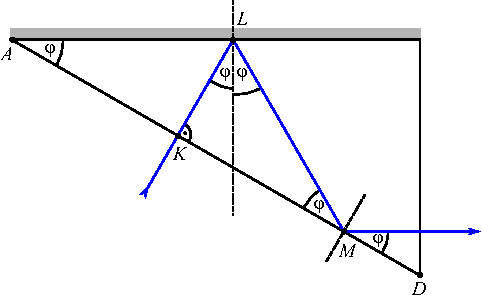
\includegraphics[width=0.65\textwidth]{2014-v3g-04-periskoopprillid_lahendus_joonis2}
\end{center}
\emph{Note}. Now that the acute angle of the prism has been found we can make certain that if a ray entering the surface perpendicularly reflects from the bottom or right face of the prism then these reflections are total. From the previous subtask it can be seen that in these cases the angle incidence is $\ang{90}-\varphi=\ang{60}$. The critical angle of a total internal reflection is $\alpha=\arcsin(1/n)=\ang{42}$. The angle of incidence $\ang{60}$ is bigger than this which means that a total internal reflection takes place.\\
\osa If a ray enters the prism from the point $B$ then the exiting ray goes through the point $D$ (see figure). \\
\emph{Note}. The direction of the exiting ray is not unequivocally determined in this case but in this solution it does not matter.\\
Using the value of $\varphi$ from the previous subtask it can be seen that the triangles $ABL$ and $BDL$ are each other’s reflections with respect to the section $BL$ (meaning that these triangles are congruent). Therefore the lengths of the sections $AB$ and $BD$ are equal from which we can conclude that $|AB|=l/2$. If a ray enters the prism from the point $C$ then it reflects straight back from the point $O$ and exits the prism from the point $C$. From right triangles we get that $|AO|=\cos(\ang{30})|AD|$ and $|AC|=\cos(\ang{30})|AO|$ meaning that the distance of the point $C$ from the point $A$ is $|AC|=\cos^2(\ang{30})|AD|=\frac{3}{4}l$. 
\begin{center}
  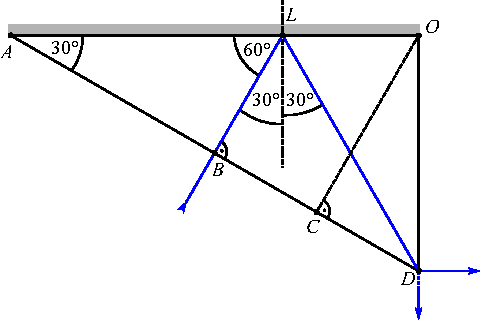
\includegraphics[width=0.65\textwidth]{2014-v3g-04-periskoopprillid_lahendus_joonis3}
\end{center}
\osa A text would be seen as a reflection if we use one plane mirror. To see the text in the right way a system has to be used where an even number of reflections take place.
\probend